\chapter{A Breakdown of all Completed Testing}
\label{appendix:testing}

\section{Round 1 Testing: Initial Classifications}
\subsection*{Testing Considerations}

I began testing the tool with three main questions. I wanted to know how the accuracy of classification is affected by:

\begin{Spacing}{1.2}
\begin{itemize}
  \item The spatial distribution of pixels chosen to create the reference curves.
  \item The temporal distribution of pixels chosen to create the reference curves.
  \item The VI used for the classification.
\end{itemize}
\end{Spacing}

To test these factors, I chose six small sample areas dispersed across Kansas, each 100 MODIS pixels square, or about 2.3 KM$^2$ (Fig. \ref{fig:studysites}). Using the USDA CDL as reference, I identified areas containing a mix of corn, wheat, soy, sorghum, and winter wheat pixels. I did my best to distribute the small areas across the state to capture a wide variety of growing conditions. This task was surprisingly difficult, given the large extent of the state and the concomitant variation in growing conditions. The crops favored tended to change from one area to another; for example, few sites in western Kansas had little more than corn and wheat.

Within each sample site, I found four to eight MODIS pixels of each of the previously listed crop types. I took care to choose only pixels in the center of fields, under the assumption such pixels would be more representative of the crop’s true temporal signature. On each chosen pixel, I digitized a vector point feature, keeping points for each crop and study area in separate shapefiles  (Fig. \ref{fig:refpoints}). I used these shapefiles as inputs to the RSG, and created two sets of reference temporal signatures for each study area: one set from the NDVI MODIS data, and another from the EVI data. I also found the mean of the signatures identified for each crop in easy study area, which gave me mean NDVI and EVI reference temporal signatures averaged across all six study sites.

I classified both NDVI and EVI data for each of the sample areas using its own reference signatures, the reference signatures derived from each of the other sample areas, and the mean signatures from all of the sample areas. This allowed me to test how the spatial distribution of pixels used to construct reference signatures affects the accuracy of classification, and which of these two VIs performs better. My initial hypothesis was that averaging signatures across multiple sites would decrease the “truthfulness” of the reference signatures because of geographical discrepancies in season start date, maximum VI intensity, and/or season length. If reference signatures are usable between study areas, but averaging multiple sites together does in fact negatively affect the derived reference curves, I expected to see rather consistent classification accuracies independent of the reference signature set used, but that the mean reference signatures produced a lower classification accuracy than those derived from single sample sites. However, if reference signatures are not useable between study areas, I expected low accuracies when the reference signatures from different study areas are used for classification, while the mean reference signatures should perform somewhere between those of the study area in question and those of the other study areas. If spatial distribution has no effect, my expectations was that the classification accuracies would be relatively consistent no matter which reference signature set is used.

I knew these tests would not directly answer my question about temporal variation in the construction of reference temporal signatures. To get an accurate answer, I knew I would need to repeat the above testing, replacing location with time as the key variable. However, given my hypothesis about the effects of spatial variation, I wanted to find out my results before devising this test. If I found the spatial distribution of pixels negatively affected the classification accuracies, then I could reasonably conclude adding a temporal component would have a similar outcome, as temporal variance would also introduce discrepancies in season start date, maximum VI intensity, and/or season length. In such a case, additional testing of this parameter would not be necessary to proceed.

\begin{figure}
  \centering
  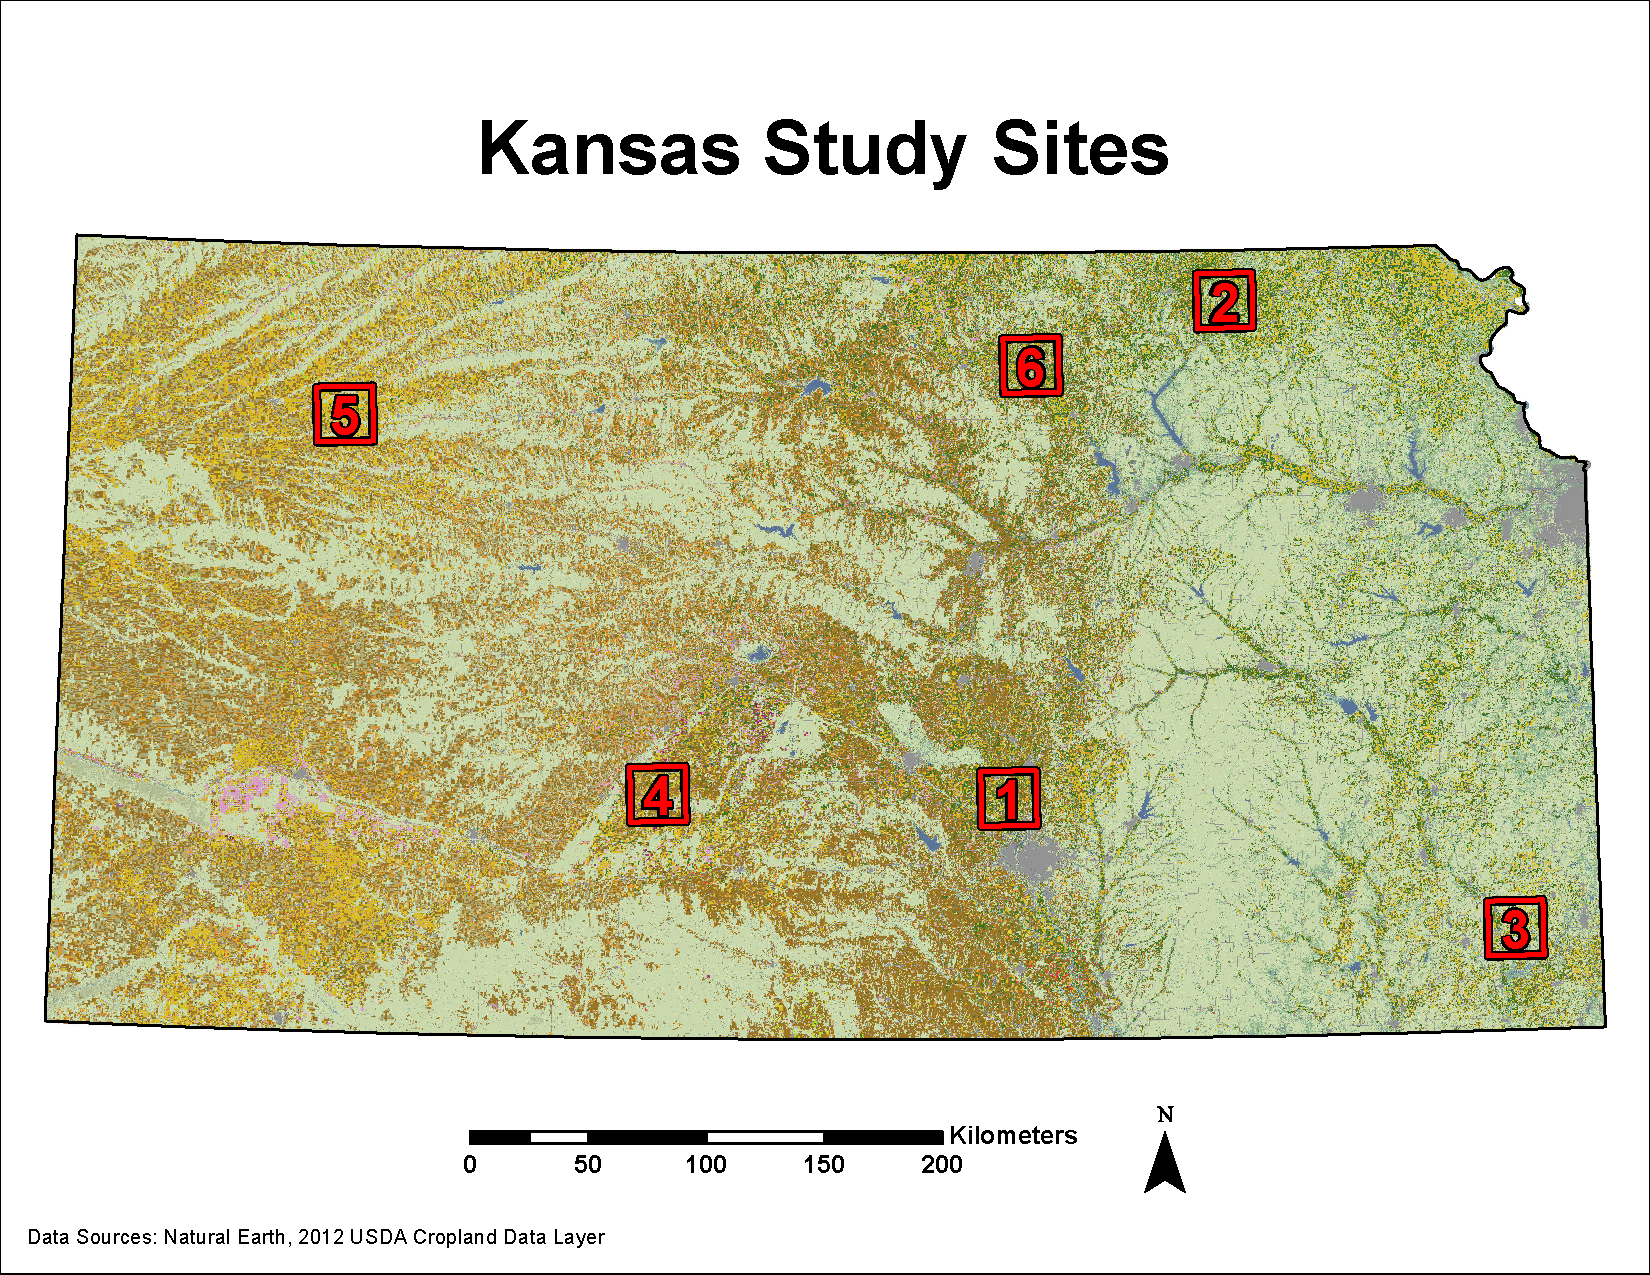
\includegraphics[width=.9\textwidth]{Graphics/Testing/STUDYSITES.pdf}
  \caption{The six study sites in Kansas.}
  \label{fig:studysites}
\end{figure}

\begin{figure}
  \centering
  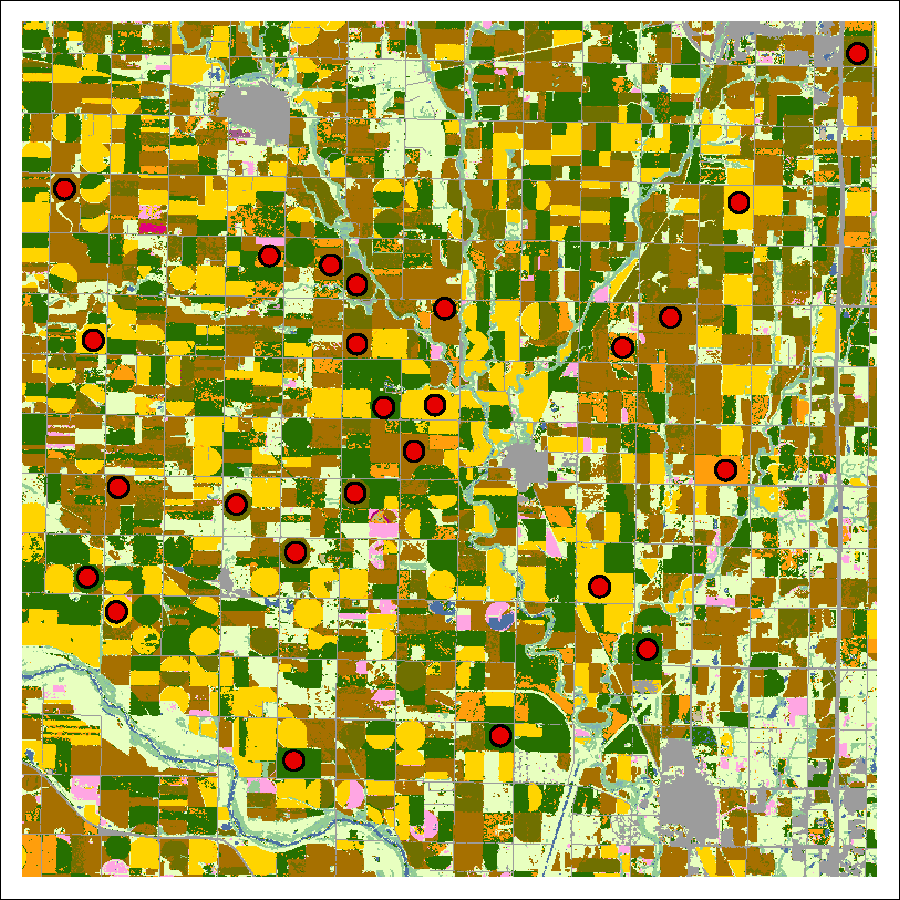
\includegraphics[width=.7\textwidth]{Graphics/Testing/clip1_30mCDL_smpl_old.pdf}
  \caption{Points dropped on pixels to use for reference signatures in study site 1.}
  \label{fig:refpoints}
\end{figure}

\subsection*{Round 1 Results and Discussion}
\label{appendix:testing:r1:results}

Some clear patterns pop out when reviewing Table \ref{table:round1results}. First, a quick scan of all the values shows that none of the classifications had a very high degree of accuracy, though study site 3 stands out with much higher accuracies than the rest. A more detailed examination of of study site 3’s results shows that the increased accuracy is due to the fact that relatively few of the pixels in the sample site are crop pixels, and a high accuracy can be achieved by not classifying the majority of the pixels, such that they are considered “other.” A breakdown of highest accuracy sample site 3 classification, that using sample site 3’s reference signatures and NDVI data, is shown in Table \ref{table:round1ss3acc}. One can see the relative abundance of “other” pixels that skews the accuracy upward compared to the other sample sites.

\begin{Spacing}{1.0}
\begin{table}
  \centering
  \caption{Overall Percent Accuracy for Each Round 1 Classification, by Sample Site (SS).\newline~Green cells indicate highest accuracy for each sample site.}
  \label{table:round1results}
  \begin{tabu}{ZZZZZZZZ}
    \toprule
    \multicolumn{8}{c}{\textbf{EVI}} \\
    \midrule
    & \multicolumn{7}{c}{Reference Signatures Source} \\
    & SS 1 & SS 2 & SS 3 & SS 4 & SS 5 & SS 6 & Mean \\
    \midrule
    SS 1 & \cellcolor{LimeGreen}55.61 & & 45.34 & 54.36 & 43.83 & 49.06 & 49.63\\
    \rowcolor{light-gray}SS 2 & 53.11 & \cellcolor{LimeGreen}64.93 & 50.00 & 47.86 & 40.79 & 42.60 & 53.69 \\
    SS 3 & 73.87 & 69.40 & \cellcolor{LimeGreen}75.23 & 73.53 & 70.57 & 71.86 & 73.71 \\
    \rowcolor{light-gray}SS 4 & 50.42 & 45.54 & 49.26 & \cellcolor{LimeGreen}53.46 & 45.30 & 49.66 & 52.54 \\
    SS 5 & 42.05 & 45.62 & \cellcolor{LimeGreen}56.00 & 54.68 & 55.06 & 49.02 & 40.29 \\
    \rowcolor{light-gray}SS 6 & 47.78 & 48.66 & 38.43 & 47.53 & 41.60 & \cellcolor{LimeGreen}49.55 & 48.44 \\
    \bottomrule
    & & & & & & & \\
    & & & & & & & \\
    \toprule
    \multicolumn{8}{c}{\textbf{NDVI}} \\
    \midrule
    & \multicolumn{7}{c}{Reference Signatures Source} \\
    & SS 1 & SS 2 & SS 3 & SS 4 & SS 5 & SS 6 & Mean \\
    \midrule
    SS 1 & \cellcolor{LimeGreen}61.08 & 48.29 & 47.91 & 60.72 & 44.85 & 51.81 & 52.75 \\
    \rowcolor{light-gray}SS 2 & 56.08 & \cellcolor{LimeGreen}67.39 & 42.66 & 52.59 & 50.62 & 48.95 & 61.21 \\
    SS 3 & 74.88 & 71.75 & \cellcolor{LimeGreen}78.69 & 77.16 & 70.62 & 71.75 & 73.70 \\
    \rowcolor{light-gray}SS 4 & 56.30 & 42.25 & 46.89 & \cellcolor{LimeGreen}59.21 & 44.72 & 54.26 & 52.48 \\
    SS 5 & 53.57 & 48.51 & 45.93 & 62.18 & \cellcolor{LimeGreen}62.83 & 60.21 & 53.07 \\
    \rowcolor{light-gray}SS 6 & & 51.90 & 38.28 & 49.82 & 47.15 & \cellcolor{LimeGreen}55.71 & 54.36 \\
    \bottomrule
  \end{tabu}
\end{table}
\end{Spacing}

[INCLUDE THE TOP ACCURACIES OF EACH OF THE OTHER SAMPLE SITES IN TABLES]

\begin{Spacing}{1.0}
\begin{table}
  \centering
  \caption{Sample site 3 NDVI top accuracy}
  \label{table:round1ss3acc}
  \begin{tabu}{rrrrrrl}
    \toprule
     & Corn & Soy & Wheat & Other & Total & User Accuracy \\
    \midrule
    Corn & 861 & 133 & 0 & 334 & 1328 & 65\% \\
    Soy & 28 & 558 & 13 & 198 & 797 & 70\% \\
    Wheat & 2 & 4 & 23 & 37 & 66 & 35\% \\
    Other & 884 & 424 & 74 & 6427 & 7809 & 82\% \\
    Total & 1775 & 1119 & 110 & 6996 & &  \\
    Producer Accuracy & 49\% & 50\% & 21\% & 92\% &  &  \\
    \multicolumn{7}{r}{Overall Accuracy: 79\%} \\
    \multicolumn{7}{r}{Kappa: 0.49} \\   
    \bottomrule
  \end{tabu}
\end{table}
\end{Spacing}

Another pattern that stands out is that using NDVI resulted in a higher top accuracy for every sample site. The numbers are fairly close between the two, so I am hesitant to conclude that optimizations would fail to make EVI-based classifications as or more accurate than NDVI-based classifications. Nonetheless, based on these results, I have determined to continue testing with NDVI only, as it seems to perform better.

Perhaps most striking pattern in Table \ref{table:round1results} is that, aside from sample site 5 in the EVI-based classifications, the highest accuracies occurred when the reference signatures generated from a particular study site were used to classify that same study site. This is not wholly unexpected—even if temporal signatures are largely location-independent, there is likely to be some location-specific phenomena influencing the shape of the signature curves. In some cases, it appears that some of the classifications using other reference signatures were of similar accuracy, as occurs with sample site 1 when it is classified using sample site 4’s signatures (61.1 percent versus 60.7 percent). However, in other cases, the accuracy is marked lower, exemplified by sample site 1 when it is classified using signatures from sample sites 2, 3, 5, and 6 (all are around ten percent lower in accuracy).

The accuracies of the mean reference signature classifications are generally low. They are never the worst, which may suggest that it is better to average a greater number of pixels together if the representative-ness of the chosen pixels cannot be established. However, this conclusion would support a more selective and refined approach to creating reference signatures: don’t try to average out bad pixels, eliminate them in the first place.

Looking back on the scenarios I outlined in my testing considerations above, I actually found none of them completely captured the behavior shown in the results. I did not see relatively consistent classification accuracies independent of the set of reference signatures used, but I also found that the reference signatures from some sample sites did well at classifying others. The mean signatures were also somewhat in the middle, generally not doing terribly well, but sometimes coming close. The best interpretation I could make of the results is that, under the right circumstances, reference signatures can be used to classify other areas. However, the cases where the reference signatures are not portable, in addition to the low overall accuracy levels, were concerning. I began to consider that I might not be able to answer the initial testing questions; instead, I realized I needed to take a step back and better explore what factors effect the classification process.

\section{Round 2 Testing: Eliminating Mixels}
\label{appendix:testing:r2}

\subsection*{Pre-testing Investigation}

I began my Round 2 testing by diving back into my Round 1 results. I wasn’t sure exactly what I needed to test, but I knew my previous results held more clues. For the sake of simplifying my investigation, I decided to focus solely on sample site 1 for the remainder of my testing. If I could boost the accuracy of its classification, I would identify some of the factors influential in the classification process. I chose sample site 1 over the others as it has the best variety of crops in which I am interested, and also includes some large non-crop areas of different land cover types. This mix seemed to offer the best testing environment of my six sites.

I first studied the classification results for sample site 1 from Round 1 produced with its own reference signatures (Fig. \ref{fig:ss1r1class}). I noticed that the major patterns generally matched the CDL fairly well. If the classification \textit{looks} correct, however, where were the errors? Obviously there should be many incorrect pixels, as this classification only had an accuracy of about 61 percent. Yet they weren’t obvious at first glance.

\begin{Spacing}{1.2}
\begin{figure}
  \centering
  \begin{subfigure}[t]{.475\textwidth}
    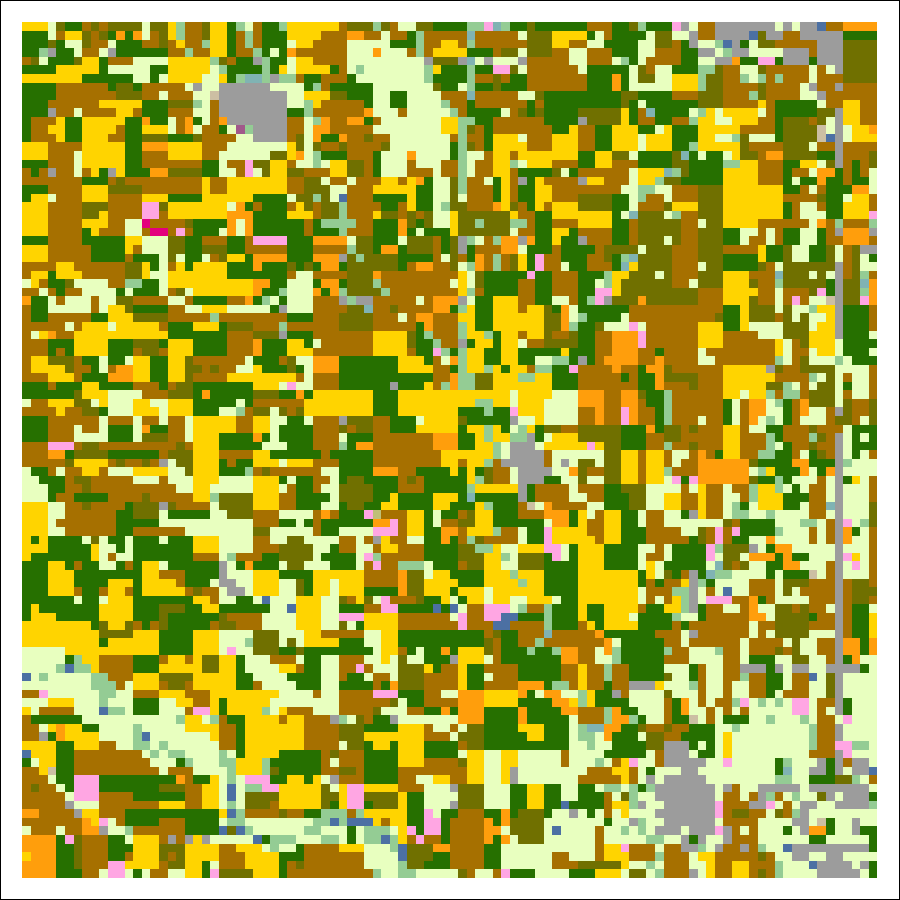
\includegraphics[width=\textwidth]{Graphics/Testing/clip1_MODIS_CDL.pdf}
    \caption{The 2012 CDL.}
    \label{subfig:ss1r1CDL}
  \end{subfigure}
  \quad
  \begin{subfigure}[t]{.475\textwidth}
    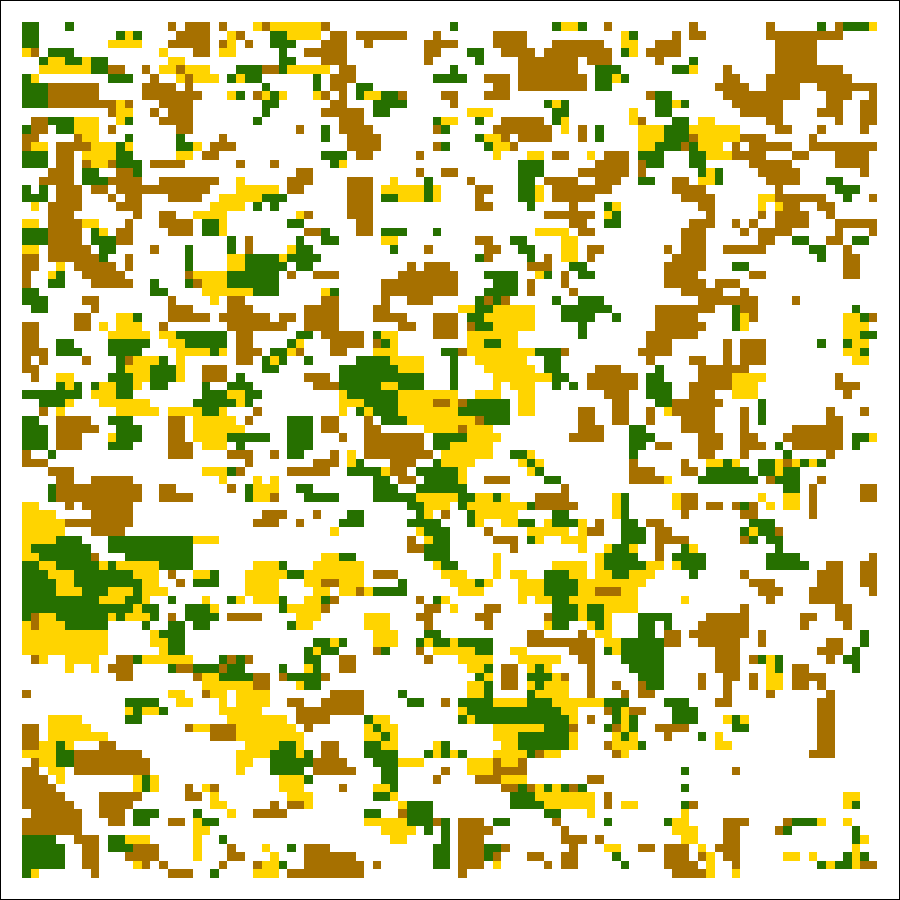
\includegraphics[width=\textwidth]{Graphics/Testing/clip1_MODIS_round1.pdf}
    \caption{Round 1 classification using SS 1 signatures.}
    \label{subfig:ss1r1class}
  \end{subfigure}
  \\
  \vspace{.25in}
  \begin{subfigure}[b]{.475\textwidth}
    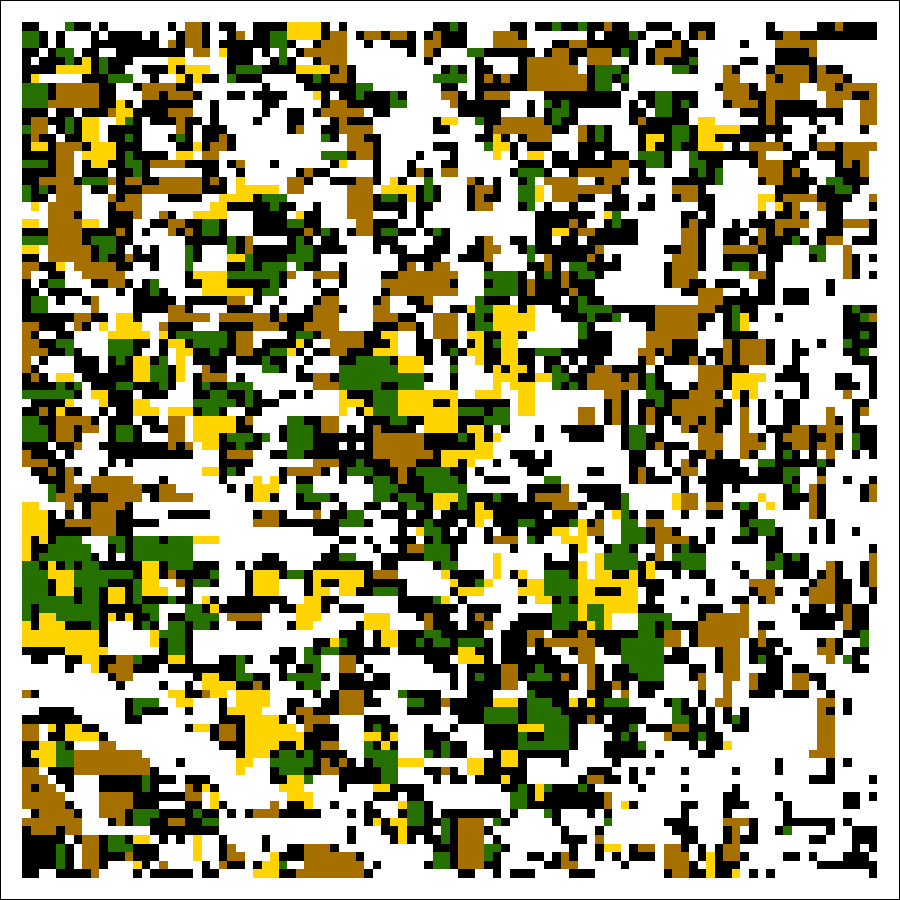
\includegraphics[width=\textwidth]{Graphics/Testing/clip1_MODIS_round1_correct.pdf}
    \caption{Correctly classified pixels. Incorrect pixels in black.}
    \label{subfig:ss1r1correct}
  \end{subfigure}
  \quad
  \begin{subfigure}[b]{.475\textwidth}
    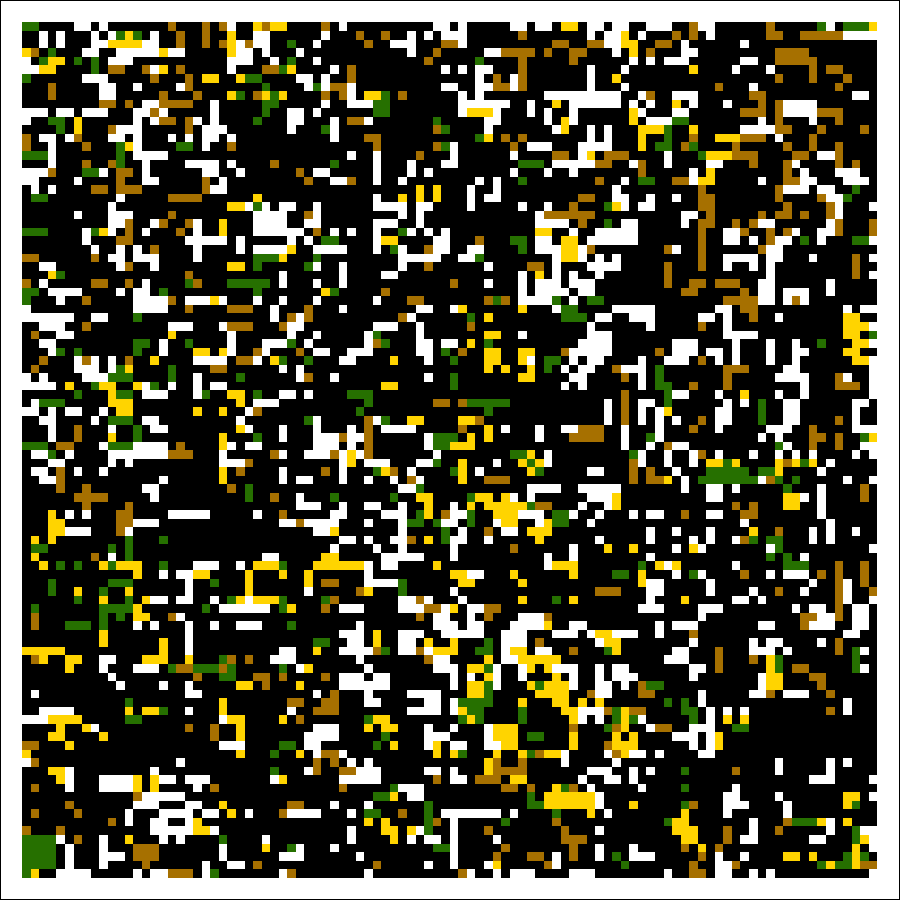
\includegraphics[width=\textwidth]{Graphics/Testing/clip1_MODIS_round1_incorrect.pdf}
    \caption{Incorrectly classified pixels. Correct pixels in black.}
    \label{subfig:ss1r1incorrect}
  \end{subfigure}
  \caption{Sample Site 1, Round 1 classification.}
  \label{fig:ss1r1class}
\end{figure}
\end{Spacing}

To find these incorrect pixels, I created two images: an image with the incorrect pixels masked in black, and an image with the correct pixels masked in black (Figs. \ref{subfig:ss1r1correct} and \ref{subfig:ss1r1incorrect}). In the former, I noticed that many of the incorrect pixels seemed to fall on the edges of fields. In the latter, I noticed some class confusion, a finding reinforced by the confusion matrix for this classification (Table \ref{table:ss1r1acc}).

The class confusion seemed to be a problem, but how to begin to remedy it was not immediately obvious to me. That so many border pixels were incorrectly classified, conversely, suggested to me that this classification method struggles when pixels have more than one land cover. Such pixels are often termed mixels.

The problem with mixels is that each land cover in a mixel has a different temporal signature. The different signatures are aggregated at the pixel level and become mixed, creating a new signature representing that specific mixture of individual signatures. This problem is not unique to my temporal data; all raster land cover data has mixels. Users of spectral data even have spectral unmixing tools to extract subpixel spectral information [TODO: CITATION].

In my case, the large size of the MODIS pixels increases their possible effect on classification accuracy. Many different land covers can be included within a 232-meter square. The large pixel size also means that a much greater percentage of the study area is composed of mixels than if a smaller pixel were used.

For these reasons, I hypothesized the low classification accuracy was becasue mixels could not be processed accurately by the fit algorithm due to the contaminated signal in a mixel curve. In other words, if two crops are mixed within a pixel, the curve of that pixel’s values from the time series image will be a blend of both crops’ phonological curves, and neither will have a good fit. Additionally, the crop which may occupy the majority of the area of the pixel may not be the largest contributor a pixel’s values; for instance, due to its high maximum VI values, a crop like soy may drive a pixel’s values up at the time of the year it is mature, even if it is in the minority of the pixel. This would further reduce the accuracy when compared to the CDL resampled by majority. Consequently, I determined I needed to find a way to removed mixels from the classification.

\subsection*{The Testing Process}

The first step in removing the mixels was to extract the MODIS raster grid from the sample site 1 TSI as vector polygons. The CDL raster is of sufficient spatial resolution (30-meter) to allow identification of fields; I converted the CDL to vector, and all continuous pixels of the same land cover value were merged into single vector features. Next, I intersected these CDL features with the pixel polygon features of the MODIS grid. From the resulting vector features I was able to select only those with an area close to that of a full MODIS pixel. Specifically, I decided to select all features greater than or equal to 53,000 m$^2$ in area (a full MODIS pixel being 53,824 m$^2$). I also manually added two [CHECK THIS] sorghum pixel features that were not selected via this process because of the low number of sorghum pixels retained. The result, shown in Fig. \ref{fig:ss1purepx}, was [TODO: INSERT NUMBER OF FEATURES HERE] features selected. These features can be thought to represent MODIS pixels which have “pure” signatures: each pixel has only one land cover contributing to its temporal signature, so each should be representative of its class.

\begin{figure}
  \centering
  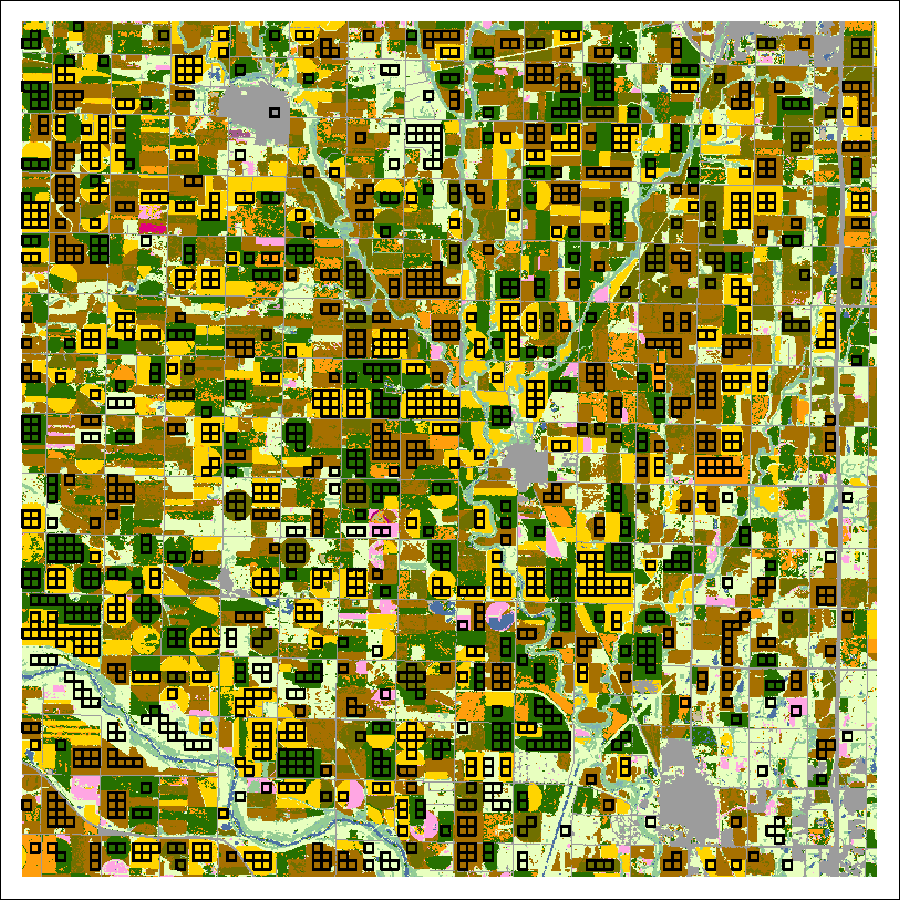
\includegraphics[width=.9\textwidth]{Graphics/Testing/clip1_30mCDL_pure_pixels.pdf}
  \caption{The pure pixels in Study Site 1.}
  \label{fig:ss1purepx}
\end{figure}

To allow me to classify only these pure pixels, I found the centroid of each of the selected pixel polygon features. The subset option of the Find Fit Tool allowed me to specify a shapefile of point features, which were converted to a list of pixel coordinates from the TSI; the tool then found the fit of the pixels in this list only. All the other pixels were assigned the  no data value. All other classification steps were the same as in Round 1, except the no data values in the fit rasters were ignored by the Classify tool when considering accuracy.

\begin{Spacing}{1.0}
\begin{figure}
  \centering
  \begin{subfigure}[t]{.63\textwidth}
    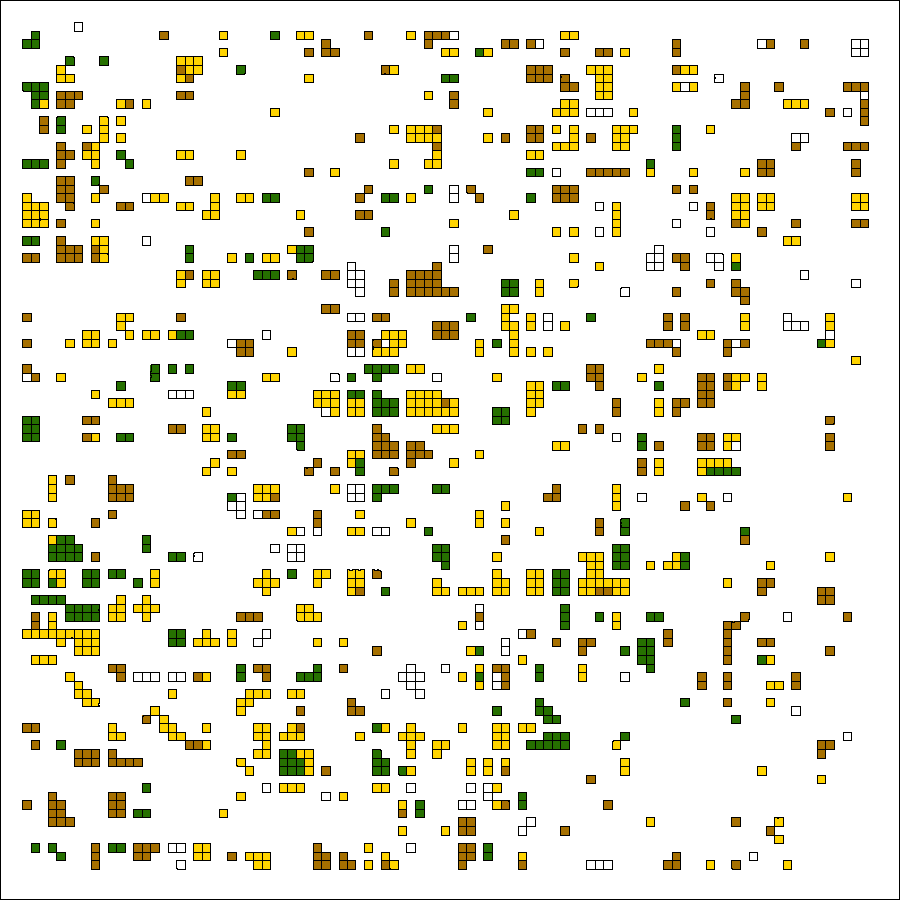
\includegraphics[width=\textwidth]{Graphics/Testing/clip1_MODIS_round2.pdf}
    \caption{The classification results.}
    \label{subfig:ss1r2class}
  \end{subfigure}
  \\
  \vspace{.15in}
  \begin{subfigure}[t]{.63\textwidth}
    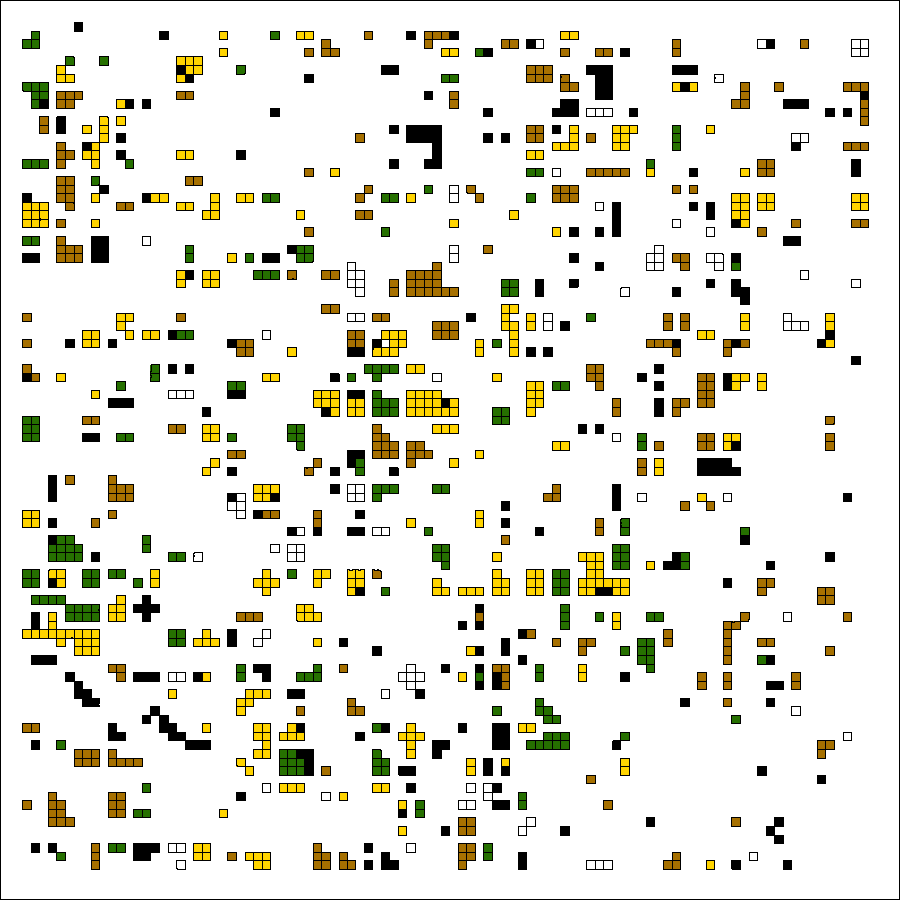
\includegraphics[width=\textwidth]{Graphics/Testing/clip1_MODIS_round2_correct.pdf}
    \caption{Correct pixels, with incorrect pixels colored black.}
    \label{subfig:ss1r2class_correct}
  \end{subfigure}
  \caption{Classification of Study Site 1 using only pure pixels.}
  \label{fig:ss1r2}
\end{figure}
\end{Spacing}

\begin{Spacing}{1.0}
\begin{table}
  \centering
  \caption{Sample site 1 NDVI: No Mixels}
  \label{table:ss1r2acc}
  \begin{tabu}{rrrrrrrl}
    \toprule
     & & \multicolumn{4}{c}{\textbf{Reference Data}} & & \\
     & & Corn & Soy & Wheat & Other & Total & User Acc. \\
    \midrule
    \multirow{4}{*}{\rotatebox{90}{\textbf{Classified}}} & Corn & 358 & 108 & 3 & 79 & 548 & 65\% \\
     & Soy & 10 & 236 & 0 & 11 & 257 & 92\% \\
     & Wheat & 36 & 6 & 348 & 29 & 419 & 83\% \\
     & Other & 10 & 4 & 20 & 101 & 135 & 75\% \\
     & Total & 414 & 354 & 371 & 220 & 1359 &  \\
     & Prod. Acc. & 86\% & 67\% & 94\% & 46\% &  &  \\
    \multicolumn{8}{r}{Overall Accuracy: 77\%} \\
    \multicolumn{8}{r}{Kappa: 0.68} \\  
    \bottomrule
  \end{tabu}
\end{table}
\end{Spacing}

\subsection*{Round 2 Results and Discussion}

The pure-pixel-only classification is shown in Fig. \ref{fig:ss1r2}, and its confusion matrix is Table \ref{table:ss1r2acc}. The confusion matrix shows the vast majority of errors are errors of commission in the corn class. Almost one third of the soy pixels and close to half of the “other” pixels are classified as corn. That corn and soy have similar signatures may suggest that those crops will always have some confusion because the similar shape and close maximum dates of early soy and late corn are not differentiable to the fit algorithm. However, if this were the issue, I would expect to see the confusion in both directions, with a greater number of corn pixels wrongly classified as soy. That the confusion is mainly one-sided led me to believe this is not the problem. Additionally, that so many “other” pixels were classified as corn suggested to me that the reference signatures I created might not be accurate.

[TODO: MAKE CSVs OF DATA AND MAKE PLOTS FOR NEXT PARAGRAPH]

I plotted the signature of each of the pixels contributing to the reference signatures [TODO: REFERENCE TO FIGURE] to see what the signatures looked like. Comparing them to the signatures shown in \citeauthor{wardlow2005state-level} revealed numerous discrepancies \mkbibparens{\citeyear{wardlow2005state-level}}. I decided that I needed to change my strategy for identifying pixels to use in making the reference signatures. Rather than simply finding pure pixels, I needed to ensure the signatures of sampled pixels were representative of the expected crop signature.

\section{Round 3 Testing: Refining the Reference Signatures}
\label{appendix:testing:r3}

ENVI has a plotting tool that allows the user to interactively select pixels in a multi band raster and view plots of the pixels’ values. This tool proved perfect for refining the reference curves, allowing me to drop points on only those pixels having an appearance matching my expectations for the crop designated by the CDL (see Fig. [TODO: INSERT REF TO FIGURE]). The new reference signatures, and the signatures of the newly-selected pixels are shown in Figs. [TODO: INSERT REFERENCE TO PLOTS]

[TODO: INSERT FIGURE OF NEW AND OLD POINTS FOR REF CURVE GENERATION]

[TODO: PLOT ENVI CURVES]

\subsection*{Round 3 Results and Discussion}

[TODO: TABLE: CONFUSION MATRIX FOR ENVI CURVES]

%[LINK TO THIS CLASSIFICATION: /Users/phoetrymaster/Documents/School/Geography/Thesis/Data/MODIS_KANSAS_2007-2012/reprojected/Classified/test1_envicurves/fullpxonly/clip1refs/classification_2014-07-29_1446/]

To my surprise, I found that refining the reference signatures actually reduced the classification accuracy to 66 percent (Table [TODO: INSERT REFERENCE TO TABLE]). I did notice almost all of the “other” pixels were correctly classified, but also that, in contrast to the Round 2 testing, errors of omission were primarily responsible for the decrease in accuracy. That is, many corn pixels in the study were classified as other. The confusion between corn and soy also remained.

To further understand what had happened, I plotted the signature of every incorrectly classified pixel in the study site. Looking through the plots, I began to notice some patterns. I found many adjacent pixels with similar plot shapes [TODO: SHOW SOME SAMPLES OF ADJACENT PIXEL SIGNATURES]. I also began to notice a few different signature shapes for each crop [TODO: SHOW SAMPLES OF REOCCURRING CROP SIGNATURES]. These two findings suggested to me that all pixels in a field generally have the same signature, and, assuming the truthfulness of the CDL, each crop has multiple temporal signatures.

The latter of these conclusions was particularly problematic to me. Not only does such reasoning conflict with previous research into phenological classification [TODO: CITE WARDLOW AND EGBERT, OTHER CROP CLASSIFICATION SOURCES], but is illogical considering the typical growth cycle for crops like corn and soy. The same crops within close proximity should be exposed to essentially equal growing conditions. Variations in planting date may account for slight differences in the temporal signatures. The use of irrigation or application of pesticides, fertilizers, or herbicides may also impart slight disparities between signatures. However, none of these variables would likely be accountable for the vastly different crop signatures observed.

To get an expert opinion, I sent a few sample signatures of incorrectly classified pixels, labeled as corn in the CDL [TODO: INSERT GRAPHICS OF THESE SIGNATURES], to Dana Peterson at the Kansas Applied Remote Sensing Program of the Kansas Biological Survey at University of Kansas. Conferring with her and her colleagues confirmed that the signatures could only be attributable to double cropping, and that the CDL is not correct in these cases.

Another class class of signatures had an unusual bump in value at the end of the year. The crop signatures shown in Wardlow/Egbert made me think the end-of-year increase in NDVI of many incorrectly classified pixel may be related to winter wheat planting for the next year’s growing season.

To investigate this idea, I used the USGS Landsat Look online imagery viewer to identify some of these incorrectly classified fields and see how they appeared through time. The fields with the increase in values at the end of the year featured vegetation throughout the winter, and had significant vegetation growth early in the following year, consistent with winter wheat. Moreover, the CDL for 2013 showed many of these fields to have winter wheat in that year (including both winter wheat/soy double cropping and winter wheat only) [TODO: CONFIRM THIS].

\section{Round 4 Testing: Different Time Ranges}

\subsection*{Deriving the Date Ranges to Test}

As many of the pixels this winter wheat bump did not fit the reference signatures within the utilized thresholds, I wondered what would happen if I changed the date range of the TSI. Instead of beginning and ending the TSI at the start of January, I decided to create a TSI that would include the end-of-year winter wheat bump from 2011 and end before the bump in 2012. Specifically, I selected images from 2011 DOY 305 through 2012 DOY 289.

[TODO: CREATE A MAP OF INCORRECTLY CLASSIFIED SHOWING 2013 WINTER WHEAT PIXELS -- %SEE /Users/phoetrymaster/Documents/School/Geography/Thesis/Data/MODIS_KANSAS_2007-2012/reprojected/Classified/test1_envicurves/fullpxonly/clip1refs/classification_2014-07-29_1446/wheat2013.tif].

As by this point I had also returned from my field work in Argentina, I had a bit better idea of how my processing procedure would have to change to classify the Pellegrini imagery. In talking with the locals, I found that wheat was just one of a number of different grains that were grown in the winter dry season, and I did not have any good way to verify where nor what types of such crops were grown in the season proceeding my travels (I was there only during the summer season). To compound the problem, I also learned that, due to the length and flexibility of the summer wet season in Pellegrini, farmers were not limited to double cropping only late summer crops with a winter crop. Instead, any summer crop could be grown with a winter crop. As I was only able to extract one double crop signature from the Kansas data, the winter wheat and soy signature, I realized I would not be able to use my Kansas signatures to classify an entire agricultural year in Argentina; I would only be able to classify summer crops. Because of this, I decided to see what would happen if I limited my sample site 1 classification to only the spring and summer months, using images from DOY 97 through DOY 273.

\subsection*{Classification Procedures}

The only difference in the processing procedure for these two classification as compared to the previous procedure in Round 3 was that I selected the desired MODIS .hdf files covering each of the date ranges and placed those files in two folders. I then used those folders as the directories for the MODIS .hdf sources when building the two TSIs. I used the same reference signatures as derived in Round 3, and only classified the pure pixels identified in Round 2.

\subsection*{Round 4 Results and Discussion}

Despite accounting for the winter wheat planting for the following year, my 2011--2012 classification was only marginally better than the full 2012 classification, achieving 68.1 percent accuracy [TODO: LINK TO TABLE]. Looking at the classification, it appears that a few of the winter wheat 2013 pixels were properly classified this time, but many remained incorrect. Evidenced by the percent accuracy, most improvements were offset by pixels now unable to be accurately classified. Given that I knew I would be focusing only on summer crops in Argentina, I did not further investigate why this was the result.

The 2012 summer-only classification fared slightly better. Given the date range, I only classified the three main summer crops---corn, soy, and sorghum---finding an accuracy of 75.1 percent. Looking at the classification and confusion matrix, I realized much of the error was due to confusion between soy and sorghum. %[SEE /Users/phoetrymaster/Documents/School/Geography/Thesis/Data/MODIS_KANSAS_2007-2012/reprojected/Summer2012/multidate_image/classification_2014-08-09_1716_5/2014-08-09_1716_2012clip1.txt]

Considering that only 18 pixels in the study area were sorghum, I tried without it, classifying just corn and soy. However, this merely traded confusion between sorghum and soy for confusion between corn and soy, maintaining more or less the same accuracy. %[SEE /Users/phoetrymaster/Documents/School/Geography/Thesis/Data/MODIS_KANSAS_2007-2012/reprojected/Summer2012/multidate_image/classification_2014-08-09_1831_11/2014-08-09_1831_2012clip1.txt]

In both summer-only classifications, I did find the accuracy to have increased, but I began to wonder if these results were directly comparable to the previous results, given that I had always been finding winter wheat, corn, and soy. To test this theory, I reclassified the 2011--2012 fit images, looking for the summer crops without wheat. Surprisingly, I found the accuracy to be exactly the same as classifying just the summer months. %[SEE /Users/phoetrymaster/Documents/School/Geography/Thesis/Data/MODIS_KANSAS_2007-2012/reprojected/2011-2012/multidate_image_1/classification_2014-08-09_1840_5/2014-08-09_1840_2012clip1.txt]
This is at least validation that restricting the classification to only the summer months does not have a negative effect on finding the summer crops. Because of this, and my working in Argentina, I decided to use the summer-only approach for all subsequent testing.

\section{Round 5: A Last Ditch Effort to Match the CDL}

In attempt to create a classification to match the CDL as best as possible, I performed a cluster analysis of the pixels of each of the crops to try to isolate the different signatures I previously identified. To begin, I created multiple masks of the TSI, each to isolate all the CDL full pixels of one of the summer crops or the wheat-soy double crop. The TSI was then processed in ENVI with each of these masks using the kmeans unsupervised classifier. Each cluster of a crop represented the different temporal signatures of that crop. I converted each pixel in the resulting clusters to vector points, organized in individual shapefiles by crop and cluster number (i.e corn3.shp is corn cluster 3). Each of these files was used with the reference curve generator tool to provide the coordinates to generate a .ref file of the mean signature for each cluster.

I used the fit tool to generate fit rasters for the .ref files, then fed them into classification/accuracy tool. That the latter tool is designed to search the fit raster names for the crop name it represents meant that using multiple fit rasters for each crop required no modifications to the code. In other words, simply telling the tool to look for “corn”, which has a value in the CDL raster of one, allowed each subset to be checked for accuracy not against itself, but against the greater whole. I determined this would provide a better means of checking the ability of the classification, as kmeans might cluster pixels together that could be better fit with another of said crop’s curves, due to the difference in the kmeans algorithm versus my fitting algorithm (e.g. it is  possible that a reference signature could be transformed to fit a pixel signature very well even if the pixel signature looks very different from the reference to the kmeans classifier).

I actually ran this processing chain twice using different cluster settings. Due to processing constraints in the classification and accuracy assessment step, I ran the first kmeans with three clusters for each crop, a 1.0 percent change threshold, and 100 iterations maximum. I considered using more clusters, but three seemed to be optimal, finding multiple signatures while keeping processing times manageable. Even using only three clusters per crop, four threshold steps, and omitting the wheat-soy double crop reference, the classification/accuracy assessment tool needed over 82 minutes to complete. Adding even one more cluster per crop would have taken almost twenty-two hours to finish.

Using the clusters for did in fact increase the classification accuracy to almost 82.5 percent, as shown in figure XXXX and table XXXX. After reviewing the results, I realized the sorghum was really not adding to the accuracy; omitting the sorghum cluster reference resulted in an ever-so-slight improvement, achieving an accuracy of 82.6 percent. It seems, especially in light of the fact that the CDL does not have clearly-delineated sorghum fields, but rather a mix of soy and sorghum, that the USDA’s classification method is unable to accurately differentiate between the two crops. Or, it could be that my method also has difficulty with these crops, given their similar temporal signatures. %[See /Users/phoetrymaster/Documents/School/Geography/Thesis/Data/MODIS_KANSAS_2007-2012/reprojected/Summer2012/kmeansTesting_2/classification_2014-07-11_1117 AND classification_2014-07-11_1639/]

One of the soy signatures had a strange, non-soy-like appearance. I decided to re-run the classifier as before, but omitting the peculiar soy signature. The accuracy did drop to 81.5 percent, but when I visually analyzed the classification I could see that all the previous errors where non-crop pixels were classified as soy were no longer present. I interpret these results to mean either that some soy fields have signatures quite similar to grassland and pasture areas, or that the CDL inaccurately classifies some grassland or pasture as soy. From my understanding of crop phenologies, and given my experience looking at crop signatures, I believe the latter is more likely.  %[See /Users/phoetrymaster/Documents/School/Geography/Thesis/Data/MODIS_KANSAS_2007-2012/reprojected/Summer2012/kmeansTesting_2/classification_2014-07-12_1612/]

When I ran the kmeans clustering a second time, I used ten clusters and 100 iterations. This clustering produced thirty clusters: ten each for corn and soy, nine for wheat-soy double cropped, and one for sorghum. Processing thirty fit rasters with the classification/accuracy tool using just two threshold values would theoretically take $0.35\times2^{30}$ seconds---almost twelve years---to complete on my computer. Rather than wait for that process to complete, I decided to use a single threshold across all the fit rasters and see what the results would be like, stepping through threshold values of 400 to 850 by increments of 50. The highest accuracy classification, 71.7 percent, occurred at with a threshold of 650 (see Table \ref{table:r5_10clust_all}). Omitting both wheat-containing reference signatures boosted the classification accuracy to 79.2 percent at the same 650 threshold value. A last test without the sorghum signature proved to be the highest accuracy at 81.0 percent, again with the same threshold of 650.

\section{Discussion and Conclusions}

Are the results still rather low because the CDL has class confusion? That is, might my inaccuracy be compounded because of inaccuracies in the CDL that my classification methods will never recreate? I must posit that my method might actually be more accurate than I can test given the problems with the CDL. However, even if the accuracy of the CDL is 90 percent, as is published, what is the a reasonable accuracy for me to achieve? If my classification were 100 percent accurate, comparing it to the CDL would only result in 90 percent accuracy. Thus, a classification of 80 percent accuracy may indeed be higher relative to the actual ground conditions. Only further testing with confirmed ground truth can really say.